\documentclass{ximera}

\title{A new Ximera Activity}
\author{MATH 425: Calculus I}

\begin{document}
\begin{abstract}
   Working with the peers in your group, solve the following problems. Make sure to show and justify all your work. Make sure everyone in the group understands the solution and participates. Be prepared to report your answers to the whole class. 
\end{abstract}
\maketitle


\begin{exercise}
    The given graph is a graph of the function $f(x)$. Use the graph to evaluate the definite integrals.
    %\includegraphics[scale=0.4]{Image files/5_1_5_2.png}
    \begin{image}
        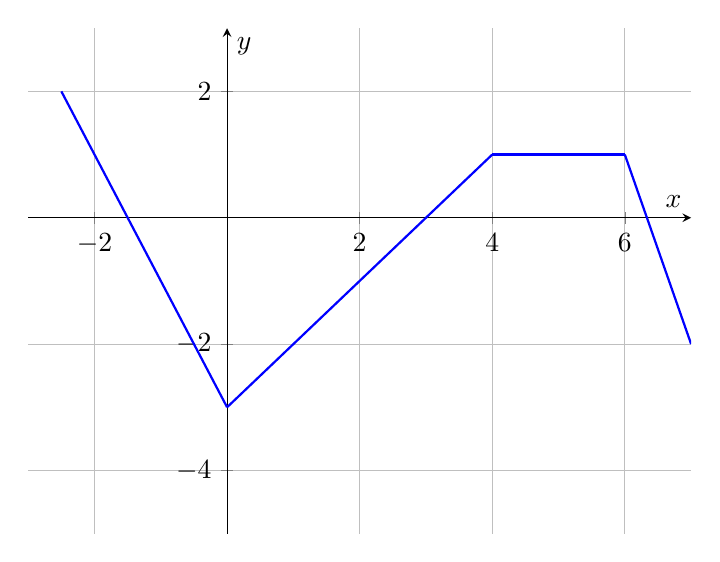
\begin{tikzpicture}
            \begin{axis}[
                axis lines = middle,
                xlabel = $x$,
                ylabel = $y$,
                xmin = -3, xmax = 7,
                ymin = -5, ymax = 3,
                grid = major,
                width = 10cm,
                height = 8cm
            ]
            
            % y = -2x - 3 for x <= 0
            \addplot[blue, thick, domain=-2.5:0] {-2*x - 3};
            
            % y = x - 3 for 0 <= x <= 4
            \addplot[blue, thick, domain=0:4] {x - 3};
            
            % y = 1 for 4 <= x <= 6
            \addplot[blue, thick, domain=4:6] {1};
            
            % y = -3x + 19 for x >= 6
            \addplot[blue, thick, domain=6:7] {-3*x + 19};
            
            \end{axis}
        \end{tikzpicture}
    \end{image}
       \begin{enumerate}
        \item $\displaystyle \int_{-2}^{0} f(x)dx$%{\color{blue}$=\frac{1}{4}-\frac{9}{4}=-2$}
        \item $ \displaystyle\int_{0}^3 f(x) dx$ %{\color{blue} $=-\frac{9}{2}$}
        \item $\displaystyle\int_0^4f(x) dx$ %{\color{blue} $=-\frac{9}{2}+\frac{1}{2}=-2$}
        \item $\displaystyle\int_0^6 f(x) dx$ %{\color{blue} $=-\frac{9}{2}+\frac{1}{2}+2=0$}
        \item $\displaystyle\int_3^6 f(x)dx$ %{\color{blue} $=\frac{1}{2}+2=\frac{5}{2}$}
        \item $\displaystyle\int_0^3 (2f(x)+1)dx$ %{\color{blue} $\displaystyle =2\int_0^3f(x)dx+\int_0^3 1dx=2(-\frac{9}{2})+1(3)=-9+3=-6$}
    \end{enumerate} 
\end{exercise} 
    
\begin{exercise}
    Suppose that the following information is given: 
    $$\displaystyle \int_1^3 f(x)=3,\;\;\;\int_1^3 g(x)=-2,\;\;\; \int_{-1}^1 f(x)=4$$
    Evaluate:
    \begin{enumerate}
        \item $\displaystyle \int_1^3 (f(x)-g(x))dx$ %{\color{blue} $=\displaystyle \int_1^3f(x)dx-\int_1^3g(x)dx=3-(-2)=5$}
        \item $\displaystyle \int_1^3 (2f(x)-4)dx$ %{\color{blue} $\displaystyle=\int_1^3 f(x)dx-\int_1^3 4dx=2(3)-4(2)=-2$}
        \item $\displaystyle \int_{-1}^3 f(x)$ %{\color{blue} $\displaystyle =\int_{-1}^1 f(x)dx+\int_1^3 f(x)dx=4+3=7$}
    \end{enumerate}

\end{exercise}





\end{document}
